\section{Resultados}

En esta sección compararemos el Método de la Potencia, su convergencia y como
influye realizar la Extrapolación Cuadrática en diferentes iteraciones.

También estudiaremos cómo afecta el parámetro de teletransportación a los
resultados.

Para los siguientes análisis decidimos utilizar un criterio de parada relativo.
Tomamos la diferencia relativa del resultado normalizado de la norma 2 entre
iteraciones.
% TODO: implementar error residual |A * x_n - x_n| al menos de pinta en el codigo

\subsection{Convergencia del Método de la Potencia}\label{sec:convergencia}

Nos interesa estudiar el comportamiento de la convergencia del Método de la
Potencia para utilizarla como referencia o caso base para luego incorporar la
Extrapolación Cuadrática.

En el Cuadro~\ref{tab:datasets} vemos instancias de prueba que utilizamos para
realizar las pruebas. Todos estos datasets provienen de sitios web reales
ajustándose al análisis deseado. Los consideramos representativos y
suficientemente grandes para nuestro análisis.

\begin{table}[!htbp]
    \centering
    \begin{tabular}{|r|c|c|l|} \hline
        Nombre & \# nodos & \# links & Descripción \\ \hline
        Cit-HepTh & 9912293 & 352807 & provisto por la cátedra \\ \hline
        web-Stanford & 281903 & 2312497 & grafo del sitio de Stanford \\ \hline
        web-BerkStan & 685230 & 7600595 & grafo de los sitios de Berkeley y Stanford \\ \hline
    \end{tabular}
    \caption{Datasets.}\label{tab:datasets}
\end{table}

Podemos observar que hay una gran variación entre la cantidad de nodos y links
entre los datasets. \emph{Cit-HtpTh} contiene muchos más nodos que links y
\emph{web-BerkStan} contiene la mayor cantidad de links, con una cantidad de
nodos menor.

\begin{figure}[!htbp]
  \begin{center}
    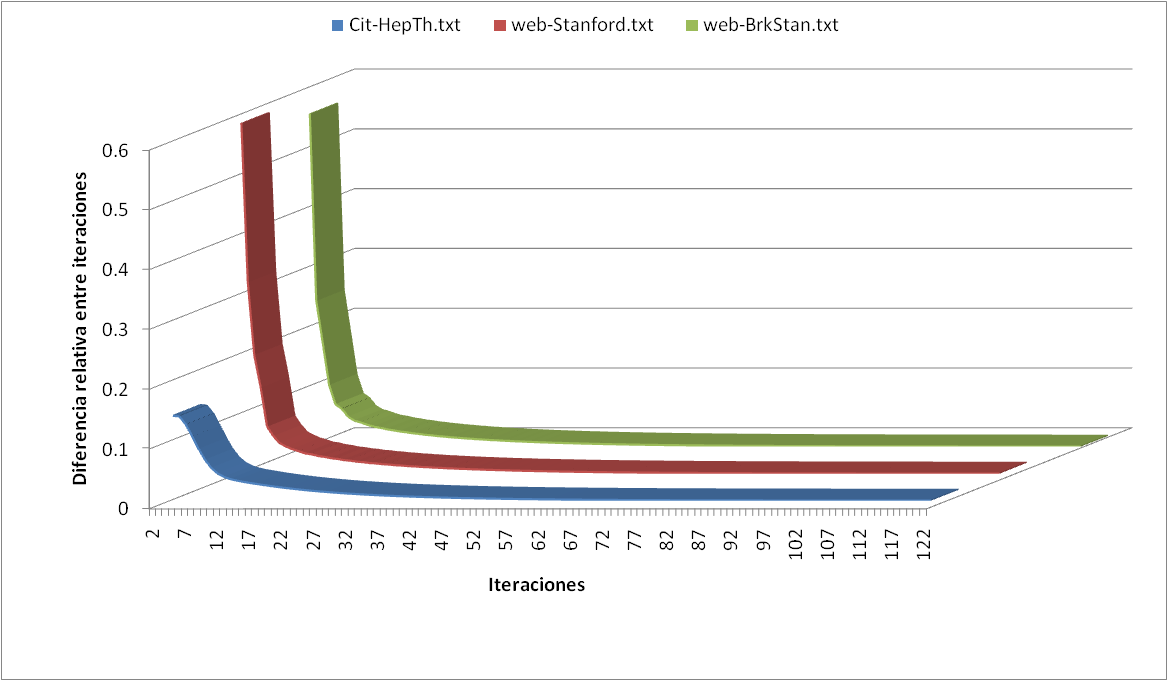
\includegraphics[scale=0.35]{img/datasets.png}
    \caption{\label{fig:datasets} Método de Potencia por instancias de pruebas.}
  \end{center}
\end{figure}

En la Figura~\ref{fig:datasets} mostramos la cantidad de iteraciones del Método
de la Potencia necesarias para lograr la convergencia deseada en el resultado.
Para esta prueba utilizamos $c=0.95$. Graficamos desde la segunda iteración
debido a que la diferencia relativa de la primer iteración es muy grande,
dejando el resto del gráfico plano.

Podemos observar que la cantidad de iteraciones necesarias para los tres
datasets es similar. Esto nos lleva a que la convergencia en los resultados es
estable y parece no verse afectados por el tamaño de la matriz, es decir, la
cantidad de nodos. Tampoco parece tener efecto la cantidad de links, ya que
todos los datasets paracen comportarse de igual forma. El tiempo de ejecución
por dataset también es similar.

Para las siguientes pruebas decidimos utilizar \emph{web-BerkStan} ya que es el
de mayor relación nodos / links, un grafo más fuertamente conexo, con mayores
relaciones entre páginas.

\subsection{Extrapolación Cuadrática}

En la Figura~\ref{fig:eq_c} mostramos el efecto de incorporar Extrapolaciones
Cuadráticas intercaladas a las iteraciones del Método de la Potencia.
Graficamos la diferencia norma 1 del resultado en cada iteración y el resultado
finalmente obtenido. Comparamos:

\begin{itemize}
    \item Sin Extrapolación Cuadrática
    \item Una Extrapolación Cuadrática en la 5ta iteración
    \item Una Extrapolación Cuadrática cada 10 iteraciones
    \item Una Extrapolación Cuadrática cada 5 iteraciones
    \item Una Extrapolación Cuadrática cada 4 iteraciones
\end{itemize}

Realizamos estas pruebas para $c=.90$, $c=.95$ y $c=.99$. Los resultados se
encuentran en las Figuras~\ref{fig:c_90},~\ref{fig:c_95} y~\ref{fig:c_99}. Por
cada variante incluímos también un detalle de la aplicación de las primeras
iteraciones con Extrapolaciones Cuadráticas en las
Figuras~\ref{fig:c_90_zoom},~\ref{fig:c_95_zoom} y~\ref{fig:c_99_zoom}.

Se puede ver claramente un acercamiento más veloz al resultado en las
iteraciones donde se realizaron Extrapolaciones Cuadráticas. Se observa también
que al menos en el inicio (las primeras iteraciones) realizar una Extrapolación
Cuadrática cada 10 iteraciones es la variante que más rápidamente converge.

\begin{figure}[!htbp]
    \centering
    \subfigure[$c=0.90$]{
        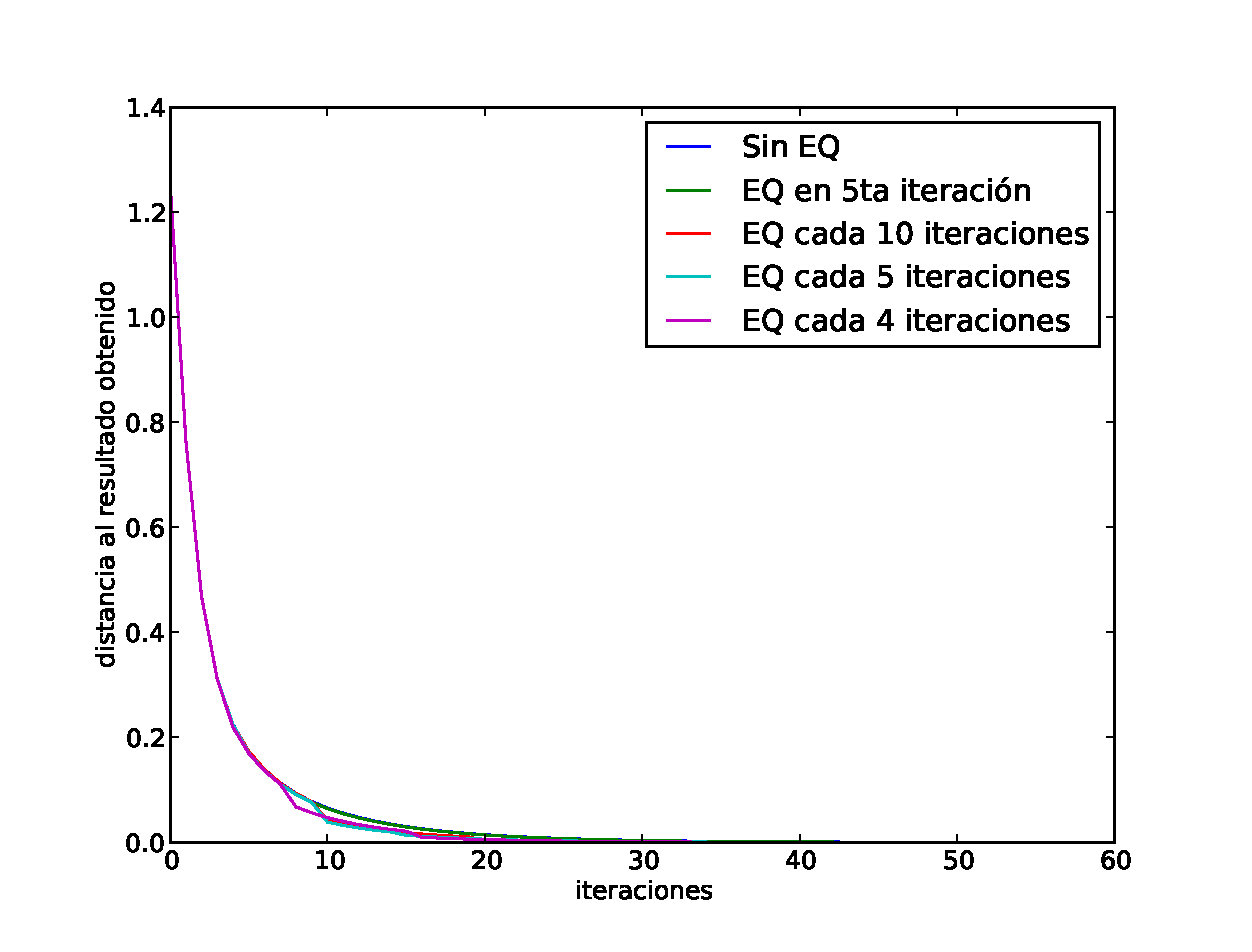
\includegraphics[scale=0.33]{img/c_90.eps}\label{fig:c_90}
    }
    \quad
    \subfigure[$c=0.90$ detalle]{
        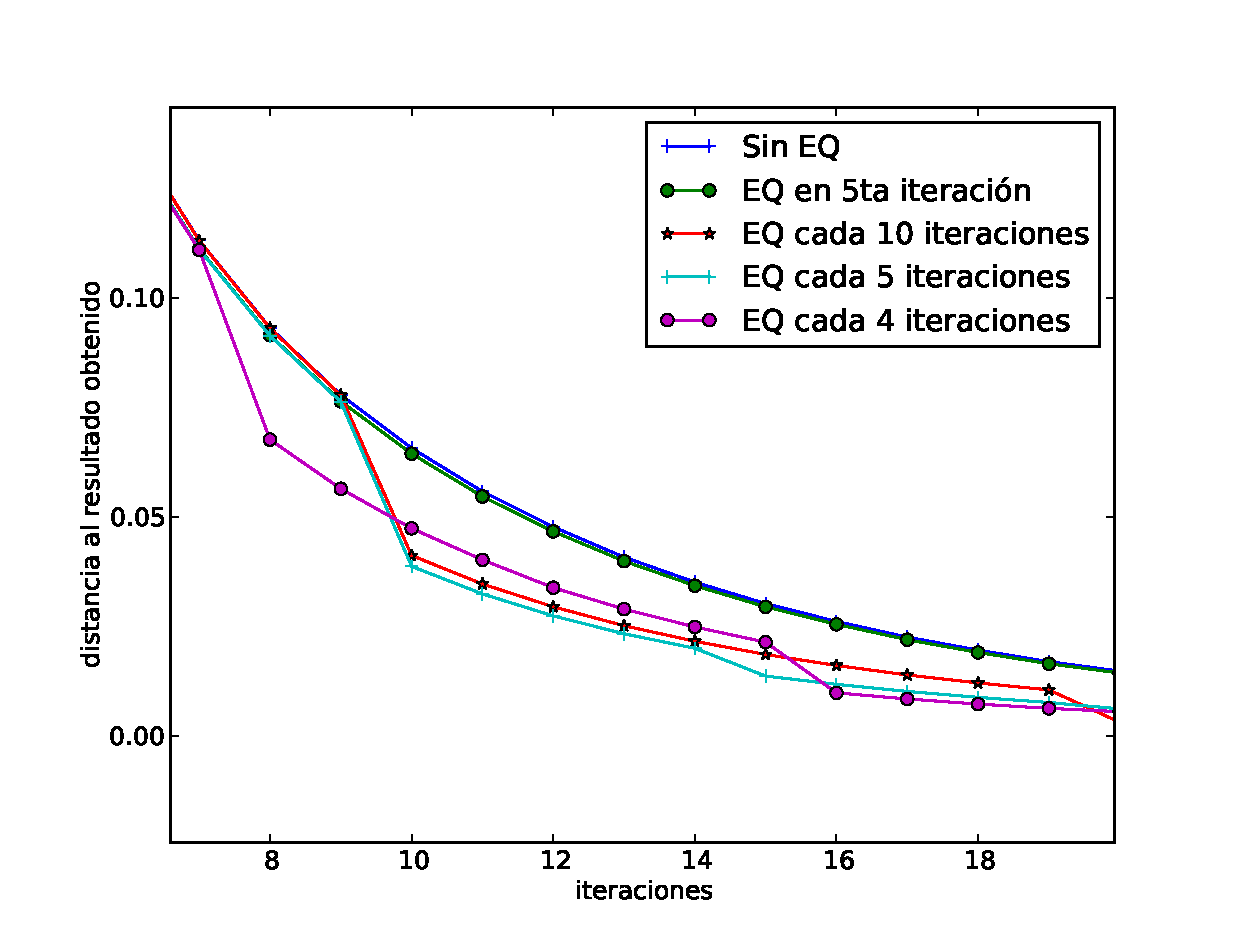
\includegraphics[scale=0.33]{img/c_90_zoom.eps}\label{fig:c_90_zoom}
    }
    \subfigure[$c=0.95$]{
        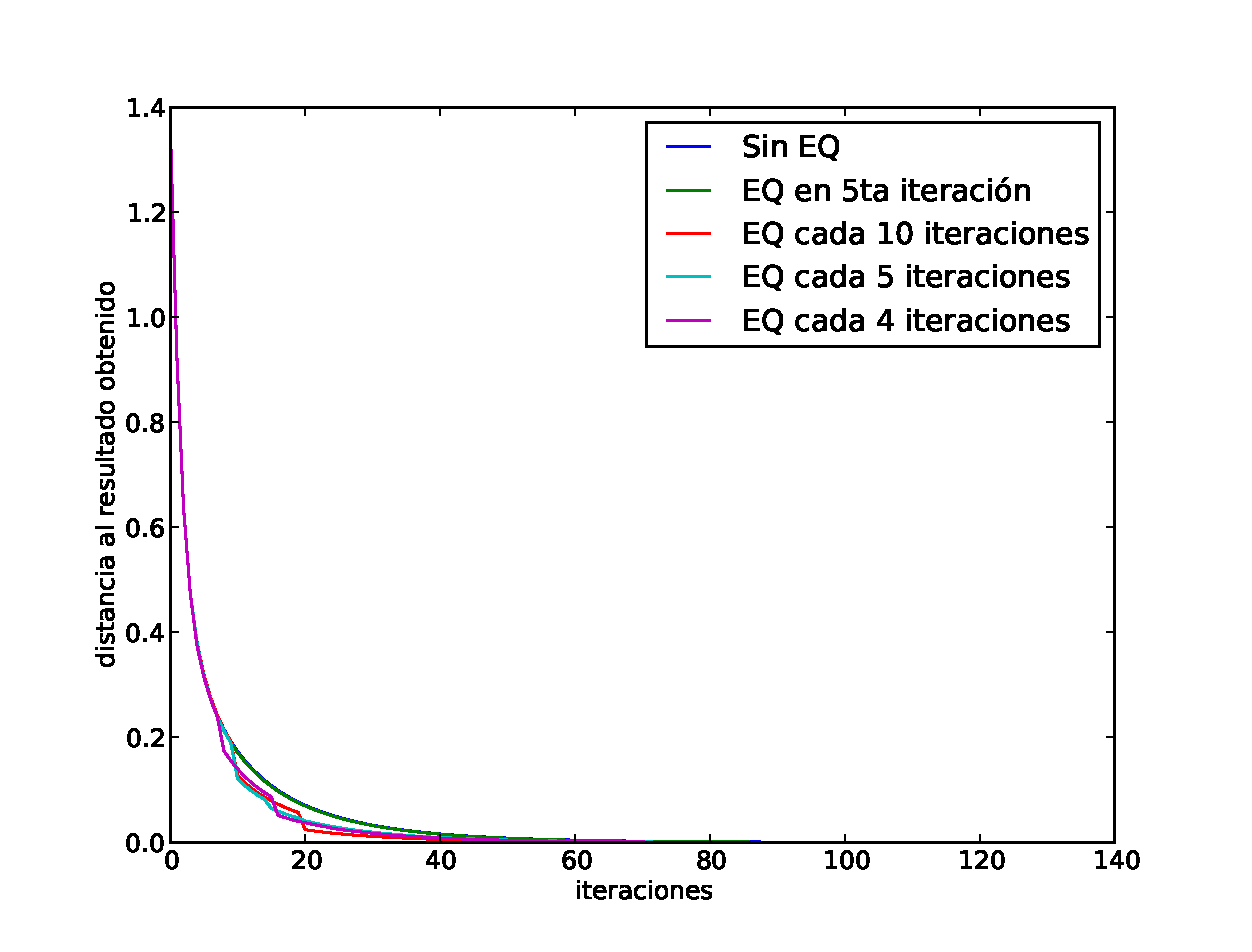
\includegraphics[scale=0.33]{img/c_95.eps}\label{fig:c_95}
    }
    \quad
    \subfigure[$c=0.95$ detalle]{
        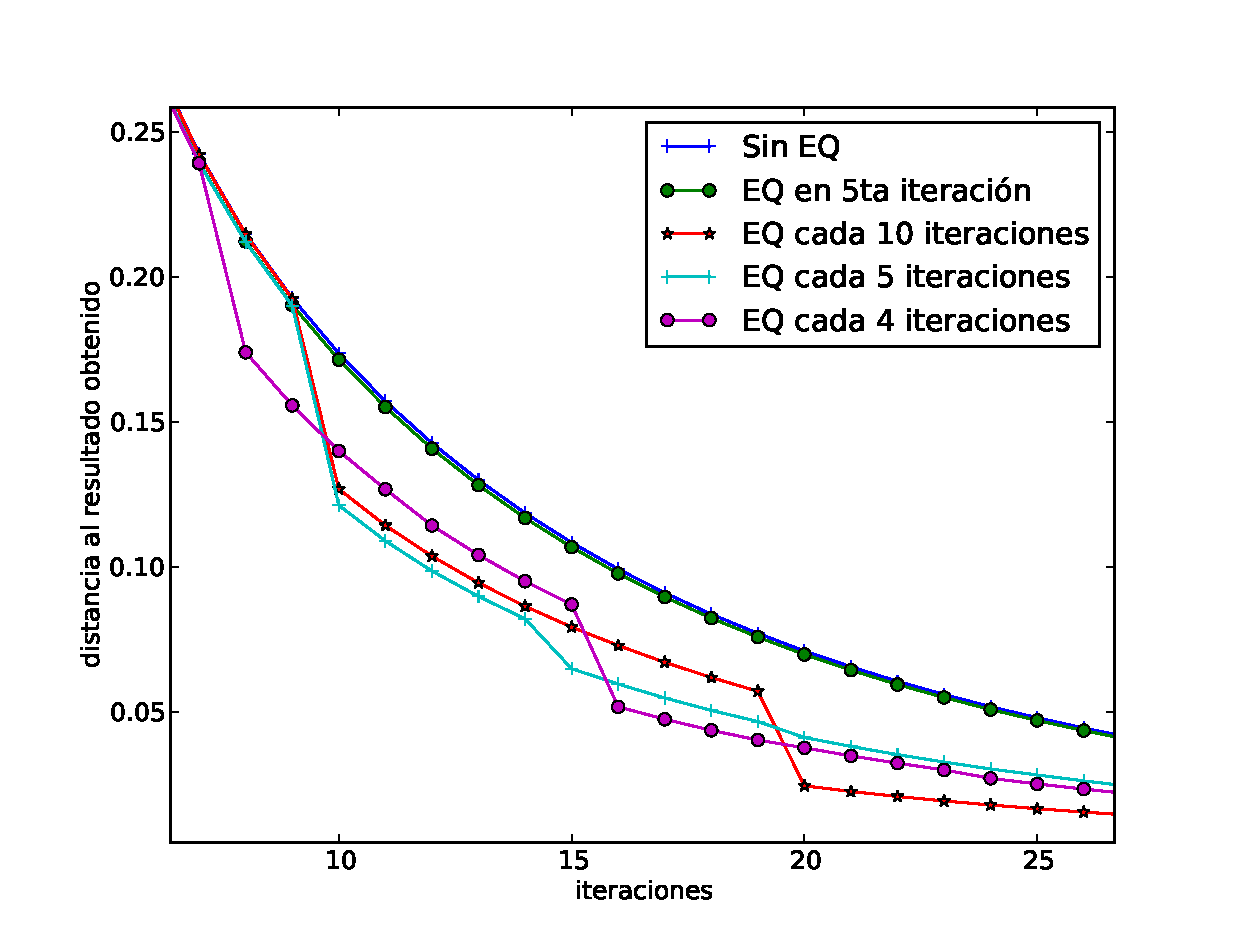
\includegraphics[scale=0.33]{img/c_95_zoom.eps}\label{fig:c_95_zoom}
    }
    \subfigure[$c=0.99$]{
        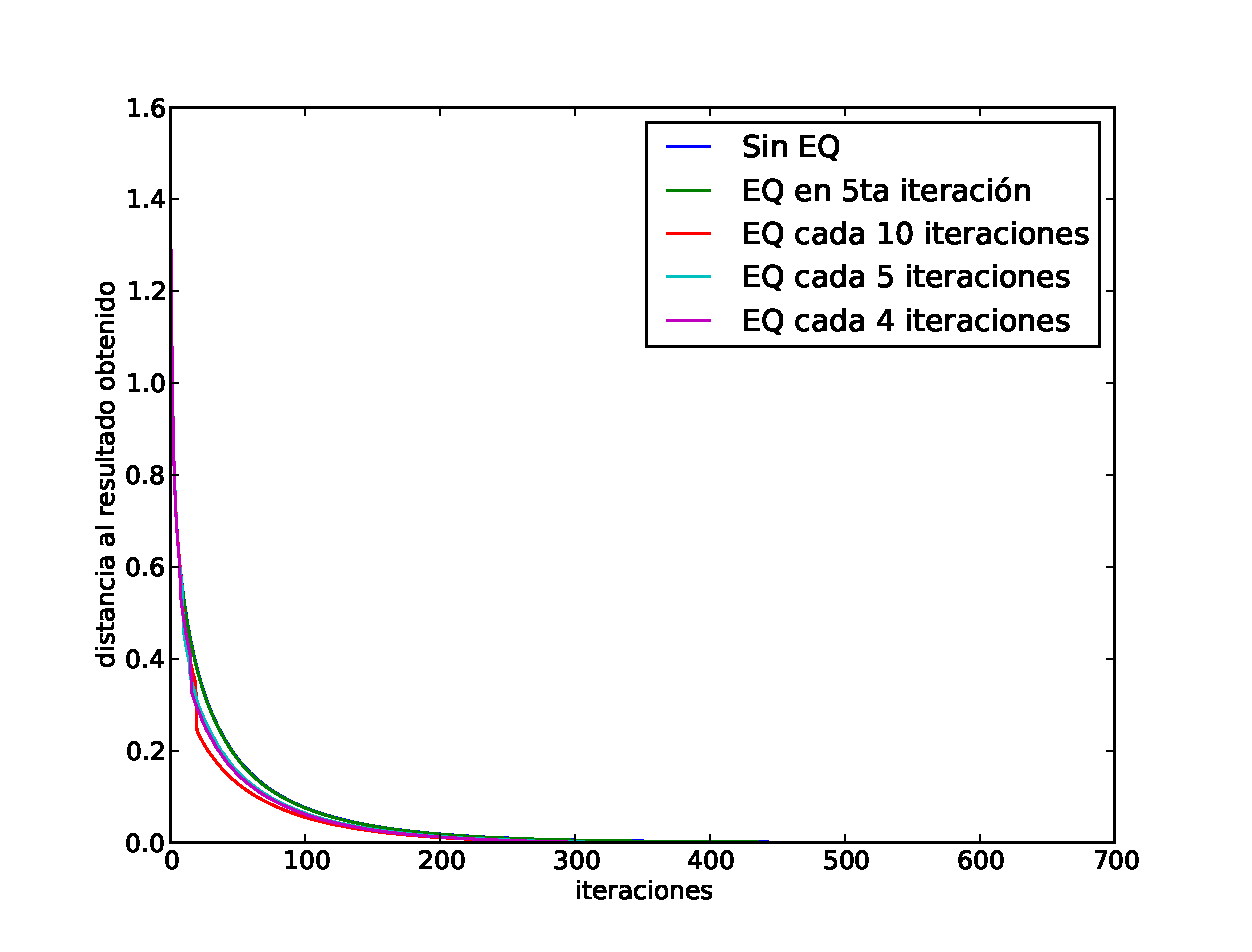
\includegraphics[scale=0.33]{img/c_99.eps}\label{fig:c_99}
    }
    \quad
    \subfigure[$c=0.99$ detalle]{
        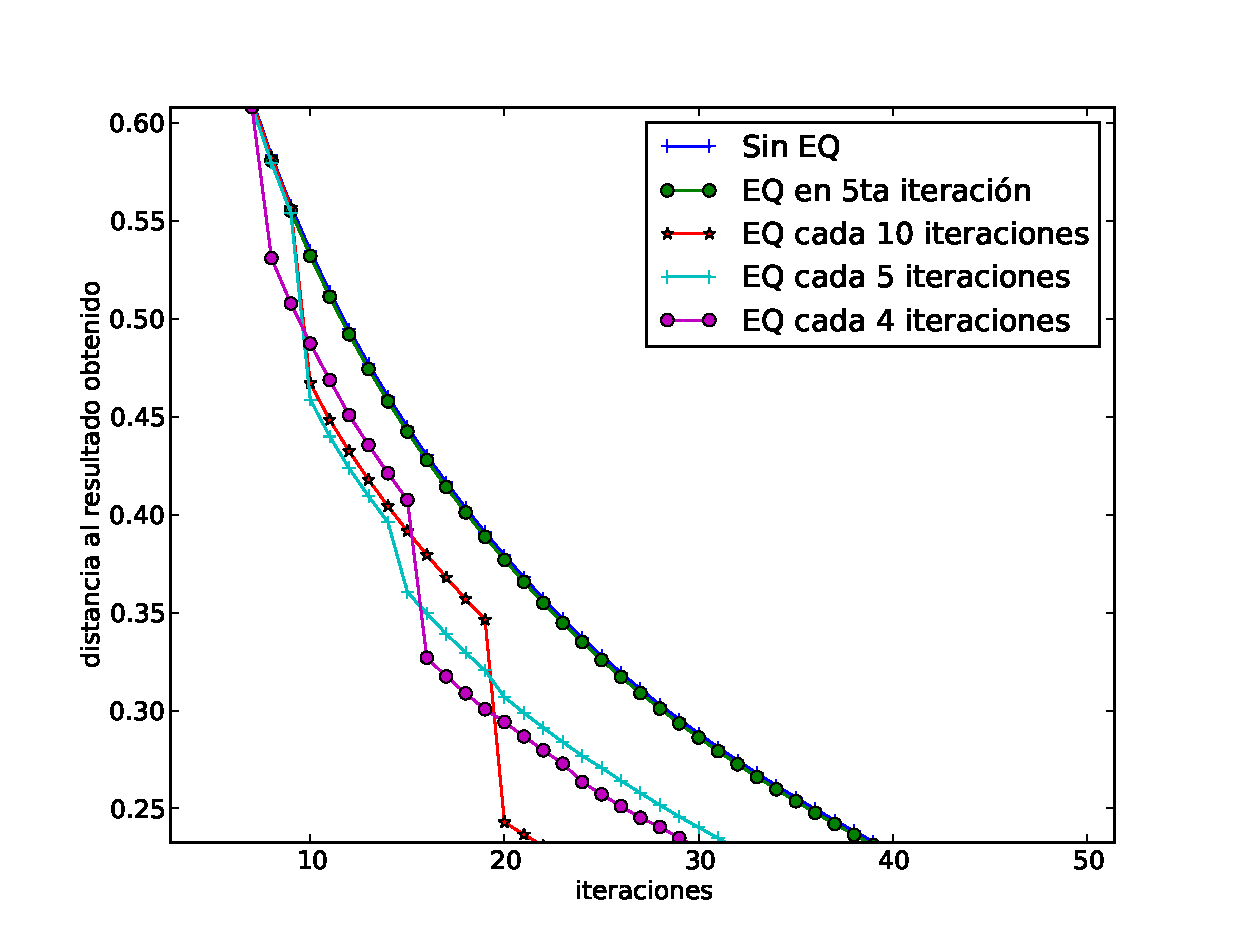
\includegraphics[scale=0.33]{img/c_99_zoom.eps}\label{fig:c_99_zoom}
    }
    \caption{\label{fig:eq_c} Mejoras aplicando Extrapolación Cuadrática en diferentes frecuencias.}
\end{figure}

Inclímos en el Cuadro~\ref{tab:iteraciones} la cantidad de iteraciones
necesarias para cada combinación de $c$ y frecuencia de iteración de
Extrapolación Cuadrática. Los datos son los mismos que los utilizados para la
Figura~\ref{fig:eq_c}. Se puede apreciar que el beneficio obtenido realizando
Extrapolaciones Cuadráticas es significativo y se encuentra en el rango de una
reducción en la cantidad de iteraciones del $27\%$ al $44\%$ para nuestro
dataset y los $c$ analizados contra no utilizar ninguna iteración con
Extrapolación Cuadrática. Incluso una sóla iteración con Extrapolación
Cuadrática produce beneficios.

Por otro lado, podemos apreciar que la convergencia del Método de la Potencia
depende del $c$ elegido. A mayor $c$ (menor grado de teletransportación) el
algoritmo requiere muchas más iteraciones para encontrar el resultado deseado.

\begin{table}[!htbp]
    \centering
    \begin{tabular}{|l|c|c|c|} \hline
                                    & $c=0.90$  & $c=0.95$  & $c=0.99$  \\ \hline
        Sin EQ                      & 59        & 122       & 676       \\ \hline
        EQ en la 5ta iteración      & 57        & 116       & 645       \\ \hline
        EQ cada 10 iteraciones      & 39        & 81        & 302       \\ \hline
        EQ cada 5 iteraciones       & 43        & 84        & 321       \\ \hline
        EQ cada 4 iteraciones       & 43        & 83        & 310       \\ \hline
    \end{tabular}
    \caption{Cantidad de iteraciones por variante.}\label{tab:iteraciones}
\end{table}
